\chapter{Przetwornik A/C typu FLASH}

\section{Programowanie transkodera RPP-S}

\begin{itemize}
        \begin{figure}[H]
            \centering
            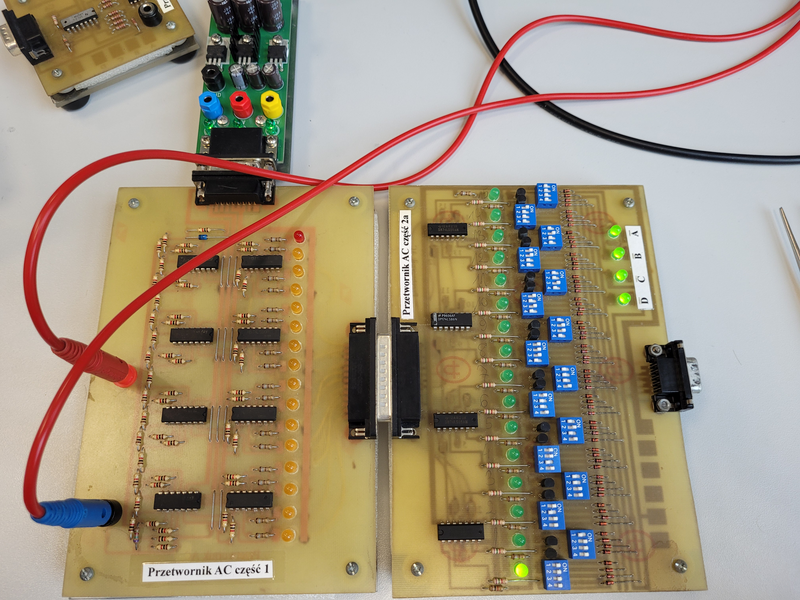
\includegraphics[width=0.7\textwidth]{img/3/20220608_105509_scaled.png}
            \caption{}
        \end{figure}
    \item Na wejście modułu podawano regulowane napięcie stałe korzystając z generatora prądu stałego.
    \item Dla podawanego napięcia zaświecały się diody na części 1 (lewy moduł), które następnie kodowano na części 2a (prawy moduł) liczbę w kodzie binarnym, którą była ilość zaświeconych diód na lewym module.
    \item Diody służące sprawdzeniu kodowania (prawa górna część prawego modułu) pokazywały \textbf{zanegowane wartości}. Należało więc uważać, aby poprawnie zakodować dane liczby.
    \item Przykładowo prawidłową wartością dla liczby $(6)_{10} = (0110)_2$ na module było:
        \begin{gather}
            \overline{A} = 1 \\
            \overline{B} = 0 \\
            \overline{C} = 0 \\
            \overline{D} = 1
        \end{gather}
\end{itemize}

\pagebreak

\section{Testowanie zaprogramowanego układu}

\begin{itemize}
    \item Na układ podawano sygnał sinusoidalny (10V, 1Hz).
        \begin{figure}[H]
            \centering
            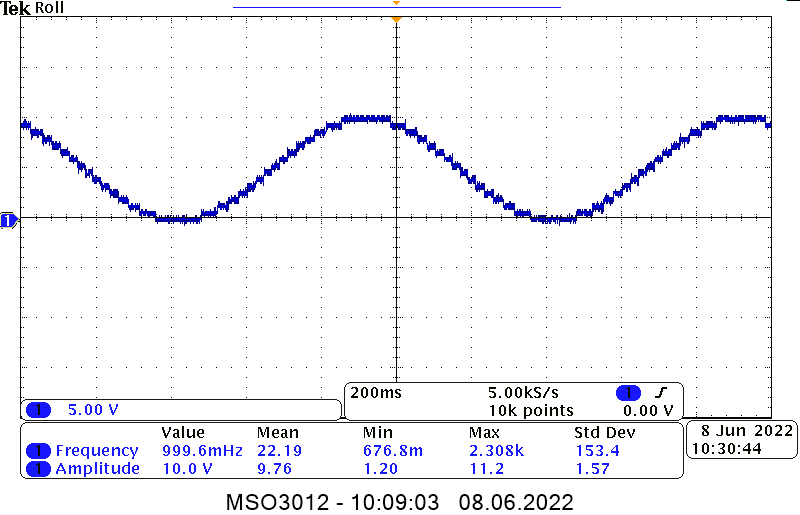
\includegraphics[width=0.65\textwidth]{img/3/3_dzialajacy_przetwornik_cropped.png}
            \label{fig:my_label}
        \end{figure}
    Układ poprawnie generował przybliżony sygnał sinusoidalny.
    \item Następnie sprawdzono reakcje układu na różne napięcia wejściowe. Ponownie przesyłano sygnał sinusoidalny o f = 1Hz.
        \begin{figure}[H]
            \centering
            \begin{subfigure}[H]{0.45\textwidth}
                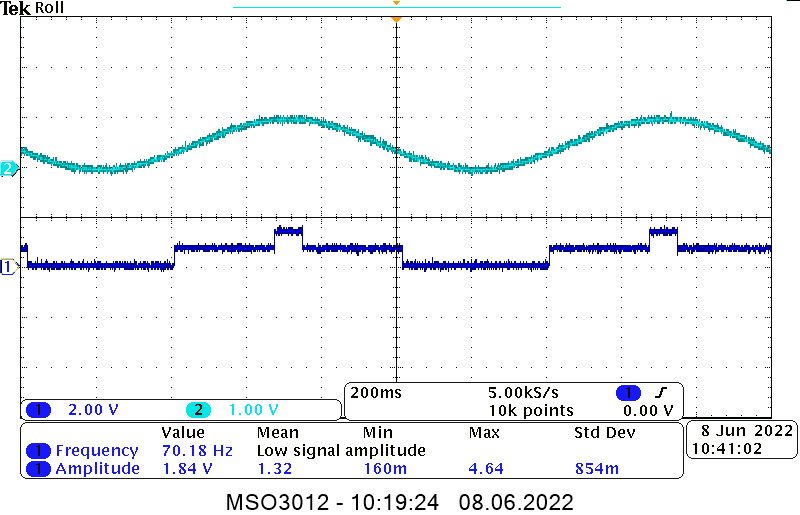
\includegraphics[width=\textwidth]{img/3/3_rozdzielczosc_1V_cropped.png}
                \caption*{U = 1V}
            \end{subfigure}
            \begin{subfigure}[H]{0.45\textwidth}
                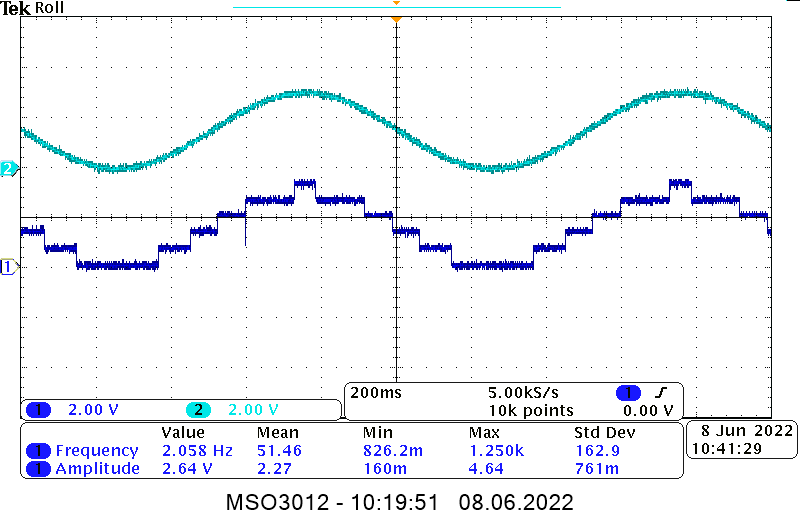
\includegraphics[width=\textwidth]{img/3/3_rozdzielczosc_3V_cropped.png}
                \caption*{U = 3V}
            \end{subfigure}
            \begin{subfigure}[H]{0.45\textwidth}
                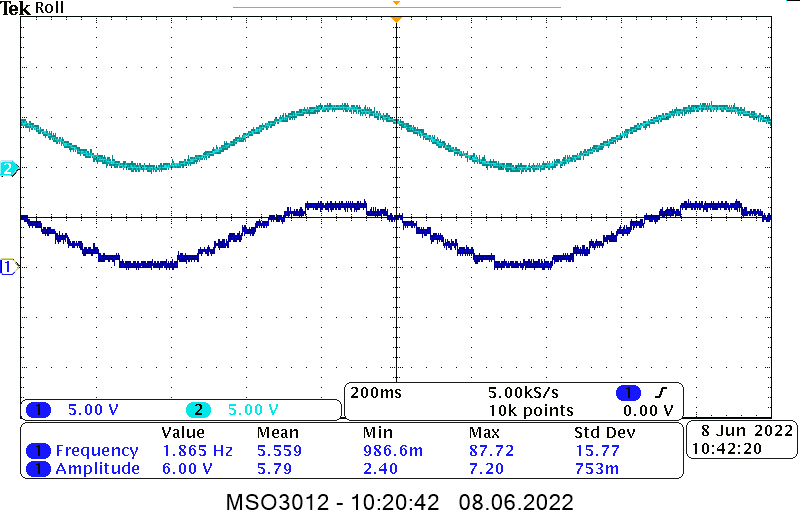
\includegraphics[width=\textwidth]{img/3/3_rozdzielczosc_6V_cropped.png}
                \caption*{U = 6V}
            \end{subfigure}
            \begin{subfigure}[H]{0.45\textwidth}
                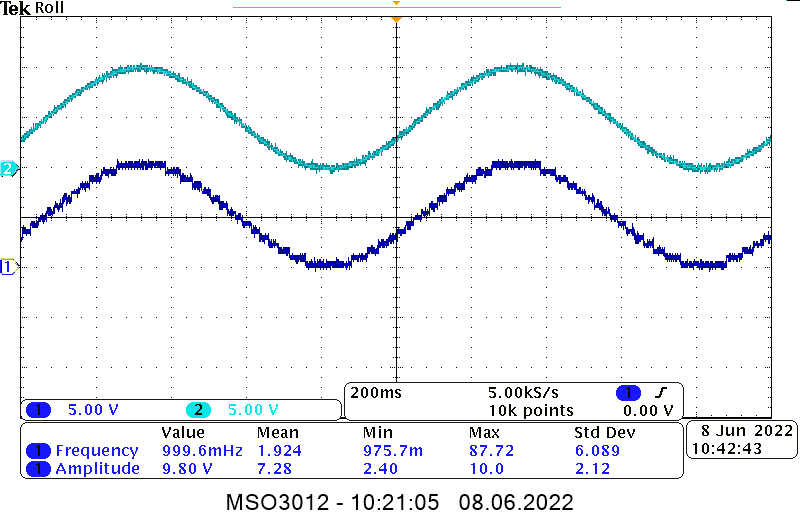
\includegraphics[width=\textwidth]{img/3/3_rozdzielczosc_10V_cropped.png}
                \caption*{U = 10V}
            \end{subfigure}
        \end{figure}
        Wraz ze wzrostem napięcia wejściowego na układ sygnał wyjściowy przypominał bardziej sygnał wejściowy.
        \item Transkoder działał poprawnie.
\end{itemize} 

\section{Programowanie modułu z pamięcią SRAM}

%20220608_113651_scaled

\begin{itemize}
    \item Zmodyfikowano konfigurację układu zmieniając transkoder RPP-S na moduł z pamięcią SRAM.
        \begin{figure}[H]
            \centering
            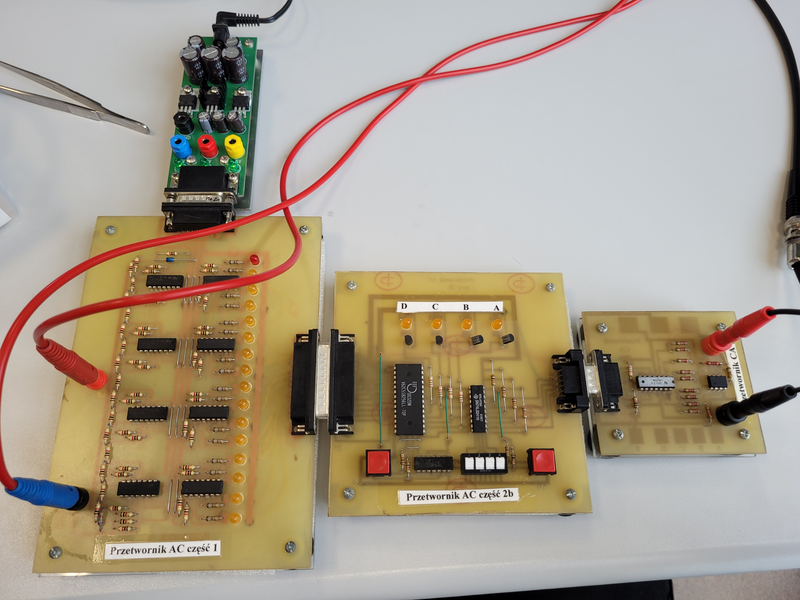
\includegraphics[width=0.9\textwidth]{img/3/20220608_113651_scaled.png}
        \end{figure}
    \item Ponownie skorzystano z generatora prądu stałego, aby generować regulowane napięcie stałe.
    \item Analogicznie do wcześniejszego modułu, podając napięcie diody na części 1 (lewy moduł) zaświecały się, następnie kodowano na części 2a (prawy moduł) liczbę w kodzie binarnym, którą była ilość zaświeconych diód na lewym module.
    \item Programowanie transkodera z pamięcią SRAM składało się na:
        \begin{enumerate}
            \item Przytrzymanie przycisku po prawej stronie - OE (output enable).
            \item Zakodowanie liczby za pomocą białych włączników.
            \item Przyciśnięcie przycisku po lewej stronie - WE (write enable).
            \item Puszczenie przycisku OE.
        \end{enumerate}
        Po każdej takiej sekwencji liczby binarne zostawały zapamiętane na module, aż do wyłączenia zasilania.
\end{itemize}

\pagebreak

\section{Testowanie transkodera z pamięcią SRAM}

\begin{itemize}
    \item Na układ podawano sygnał sinusoidalny o amplitudzie 10V oraz różnej częstotliwości:
        \begin{figure}[H]
            \centering
            \begin{subfigure}[H]{0.45\textwidth}
                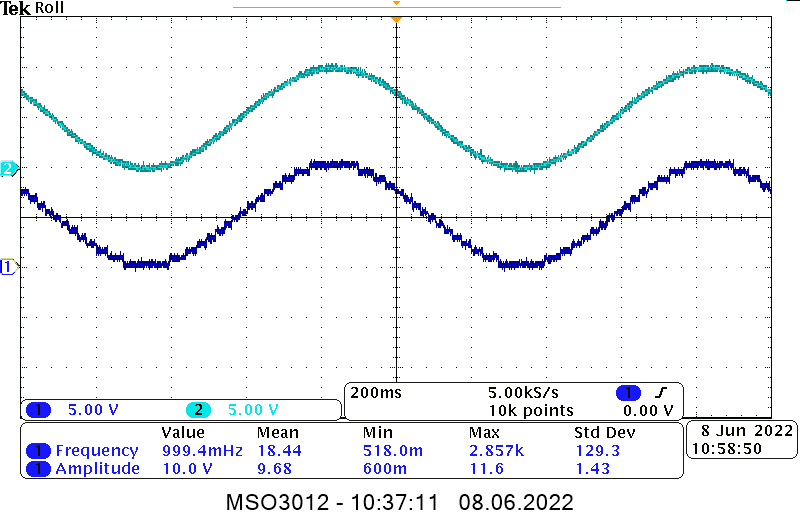
\includegraphics[width=\textwidth]{img/3/3_sram_1hz_cropped.png}
                \caption*{f = 1Hz}
            \end{subfigure}
            \begin{subfigure}[H]{0.45\textwidth}
                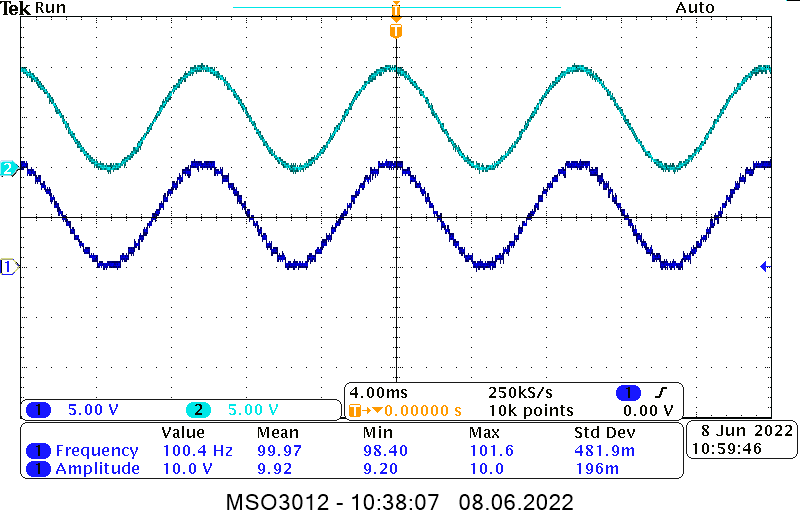
\includegraphics[width=\textwidth]{img/3/3_sram_100hz_cropped.png}
                \caption*{f = 100Hz}
            \end{subfigure}
            \begin{subfigure}[H]{0.45\textwidth}
                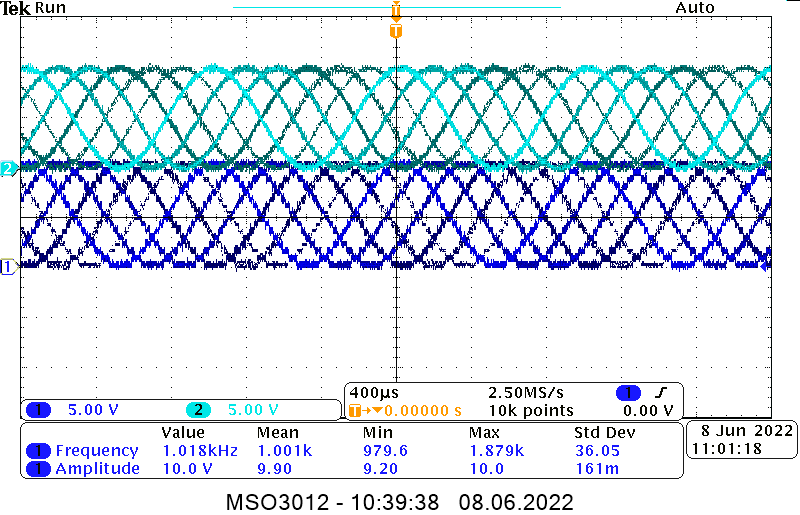
\includegraphics[width=\textwidth]{img/3/3_sram_1khz_cropped.png}
                \caption*{f = 1kHz}
            \end{subfigure}
            \begin{subfigure}[H]{0.45\textwidth}
                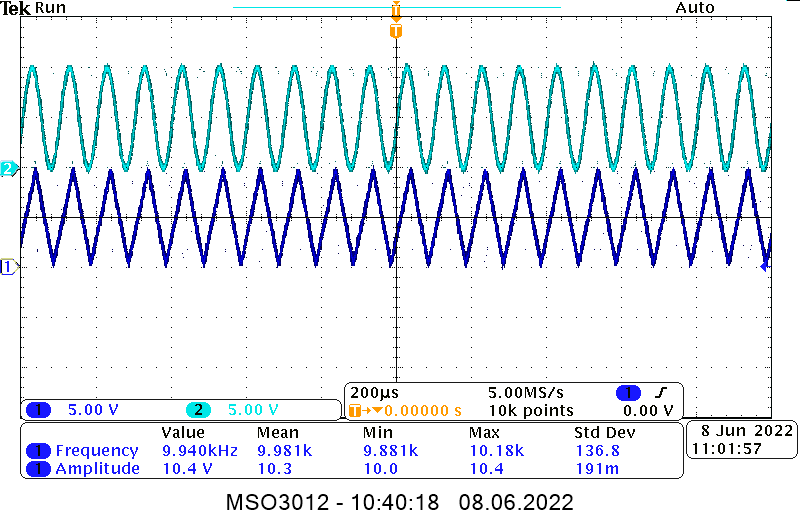
\includegraphics[width=\textwidth]{img/3/3_sram_10khz_cropped.png}
                \caption*{f = 10kHz}
            \end{subfigure}
            \begin{subfigure}[H]{0.45\textwidth}
                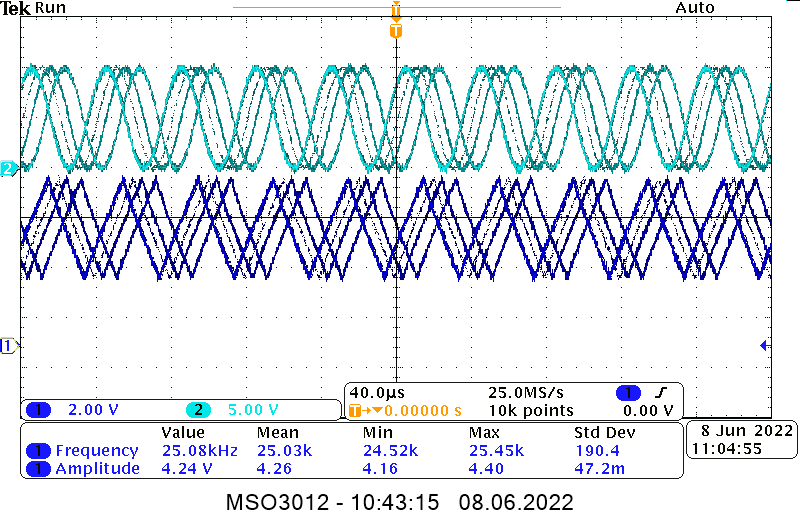
\includegraphics[width=\textwidth]{img/3/3_sram_25khz_cropped.png}
                \caption*{f = 25kHz}
            \end{subfigure}
            \begin{subfigure}[H]{0.45\textwidth}
                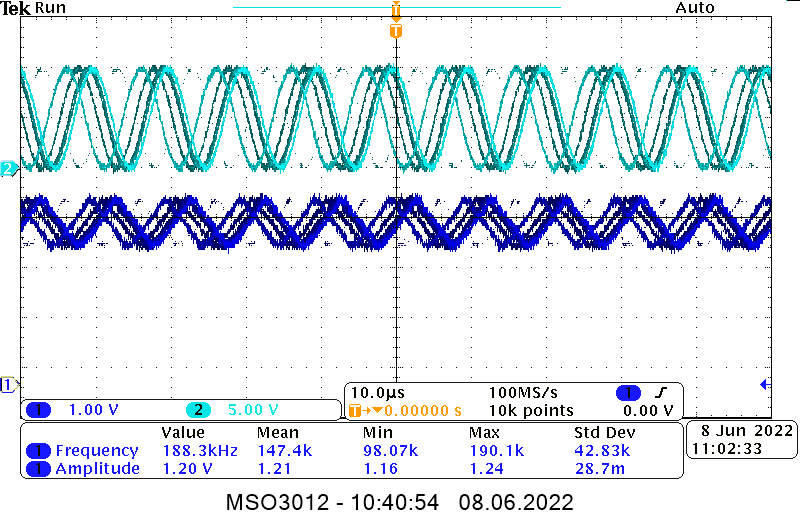
\includegraphics[width=\textwidth]{img/3/3_sram_100khz_cropped.png}
                \caption*{f = 100kHz}
            \end{subfigure}
        \end{figure}
    \item Dla wyższych częstotliwości sygnał wyjściowy zaczynał być zniekształcony. Dla częstotliwości >25kHz pozostawał on sygnałem trójkątnym o dużo niższej amplitudzie.
    \item Transkoder działał poprawnie.
\end{itemize}